\section{Discussão}
\section{Modelagem matemática de uma esfera carregada sob o campo do Van der Graff}
Conforme discutido anteriormente, duas cargas iguais exercem uma força de repulsão entre si. Podemos, então extrapolar este resultado para modelar o ângulo formado por uma esfera carregada com carga de mesmo sinal pendurada por um fio isolante há uma distância \(r\) do centro do van de Graff. Tal experimento está ilustrado na \cref{vander}

\begin{figure}[htb]
    \centering
    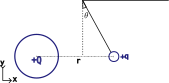
\includegraphics[width=.5\linewidth]{figs/vanderball.png}
    \caption{esfera carregada a uma distância \(r\) do van der Graff igualmente carregado pendurada por um fio isolante e formando um ângulo \(\theta\) com a vertical usualmente formada na ausência do campo elétrico}\label{vander}
\end{figure}

\begin{align*}
    {|T|} &= \frac{{|P|}}{\cos \theta}\\
    {|T|} &= \frac{{|F_{e}|}}{\sin \theta}\\
    \implies \frac{{|P|}}{\cos \theta} &= \frac{{|F_{e}|}}{\sin \theta}\\
    \implies \theta &= \arctan \left( \frac{{|F_{e}|}}{{|P|}}\right) 
\end{align*}

Podemos utilizar a lei de Coulomb para determinar a força elétrica em função da carga \(Q\) do van der Graff:
\[
    F_{e} = \frac{qQ}{4 \pi \varepsilon_{0} r^{2}}
\]
Assim, substituindo na fórmula:
\begin{align*}
    \theta &= \arctan \left( \frac{qQ}{4 \pi \varepsilon_{0}r^{2}{mg}} \right)
\end{align*}

Com isso, seria possível testar este ângulo como medida indireta da lei de Coulomb. No entanto, não pudemos realizar esta medida pela falta de uma bola e um fio isolante no lab demo.
